%!TEX root = ./main.tex
\begin{frame}[fragile]{Heap}
    
    \pause
    \begin{itemize}
        \item <2-> Vertex and edge labeled graph 
        \item <3-> Each node represents a memory cell
        \item <4-> Each edge represents a pointer/selector
        \item <5-> '\#' represents the \textit{null node}
        \item <6-> '*' represents the \textit{dangling node}
        \item <7-> Labels on nodes for variables
    \end{itemize}

\end{frame}

\begin{frame}[fragile]{Heap}
    
    \pause
    \begin{definition}
        A \textit{heap} is defined as a tuple $(\overline{M}, E, s, t, \tau, \lambda)$
        where:
        \begin{itemize}
            \item <3-> $\overline{M} = M \cup \{\#, *\}$, where $M$ is the set of memory cells
            \item <4-> $E$ is the set of edges
            \item <5-> $s : E \rightarrow M$ is the \textit{source function} 
            \item <6-> $t : E \rightarrow \overline{M}$ is the \textit{target function}
            \item <7-> $\tau : E \rightarrow C$ is the \textit{type function}, where $C = \{1, 2\}$ is the set of selectors
            \item <8-> $\lambda : X \rightarrow \overline{M}$ is the \textit{variable function}, where $X$ is a set of variables
        \end{itemize}
    \end{definition}
\end{frame}

\begin{frame}[fragile]{Heap}
    
    \pause
    Example of a heap:
    \pause
    
    \begin{figure}
        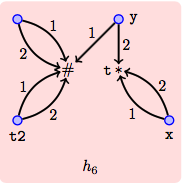
\includegraphics[scale=0.57]{images/Heap6Example.png}
        \\ \tiny{Example Heap \cite{abdulla2013monotonic}}
    \end{figure}

    \pause

    \begin{itemize}
        \item The heap invariant: 
        \item <5-> $\forall c \in C$ $\forall m \in M : |s^{-1}(m) \cap \tau^{-1}(c)| = 1$ \\
    \end{itemize}
\end{frame}

\begin{frame}[fragile]{Heap Transition System}
    
    \pause

    \begin{itemize}
        \item <2-> Subset of C includes the following operations: 
            \begin{itemize}
                \item <3-> Conditions: $x == y$, $x$ !$= y$
                \item <4-> Assignments: $x = y$, $x = y.next(i)$, $x.next(i) = y$
                \item <5-> Allocation: $x = malloc()$ and $free(x)$
            \end{itemize}
        \item <6-> The Transition System is defined as $T = (S, \rightarrow)$
            \begin{itemize}
                \item <7-> $S$ is a set of states which are pairs of $(pc, h)$ where $pc$ is the Program Counter
                \item <8-> $\rightarrow$ reflects the heap manipulation
            \end{itemize}
        \item <9-> Given states $s, s'$, $s \rightarrow s'$ exists if an operation is defined which transforms $h$ into $h'$ 
    \end{itemize}


\end{frame}

